%CONFIG DEL DOC
\documentclass[a4paper, 12pt, spanish]{article}

\usepackage[utf8x]{inputenc}
\usepackage{babel}
\usepackage{multicol, enumitem}
\usepackage{graphicx}
\usepackage{fancyhdr}
\graphicspath{ {images/} }
\usepackage{anysize} 
%\pagenumbering{gobble}

\marginsize{2.5cm}{2.5cm}{2cm}{2cm} 
\def\code#1{\texttt{#1}}


\title{Informe Trabajo Práctico N°2 \linebreak \textit{Atari Asteroids} \linebreak}

\author{Malena Díaz Falvo y Agustín Ormazábal}
\date{30 de Junio de 2019}


\begin{document}

\begin{figure}[t]
	
\includegraphics[width=8cm]{logoFIUBA} 
\end{figure}

\maketitle

\thispagestyle{empty}
\newpage

\setcounter{page}{1}
\pagestyle{fancy}
\fancyhf{}
\rhead{Algoritmos y Programación - 95.11}
\lhead{102374 - 102142}
\cfoot{\thepage}
\renewcommand{\footrulewidth}{0pt}




\section*{Introducción}
El actual proyecto consta de la implementación de una reversión del juego
Asteroids en lenguaje ISO-C99 utilizando la biblioteca gráfica SDL2. Para su recreación
se implementó el concepto de TDA, entre otras funcionalidades incorporadas a lo largo
del curso. \newline
 
\section*{Desarrollo}
Para abordarlo, se utilizaron y modificaron algunos de los archivos brindados para el TP1 (reversión del Lunar 
Lander). Además, se diseñaron y utilizaron diferentes TDAs para los objetos del juego, obteniendo finalmente los siguientes \texttt{.h}:

\begin{multicols}{2}
\begin{itemize}[label=$\bullet$]

	\item \texttt{caracteres.h}
	\item \texttt{config.h} 
	\item \texttt{dibujar.h}
	\item \texttt{diccionario.h}
	\item \texttt{movimiento.h}
	\item \texttt{nave.h}
	\item \texttt{asteroides.h}
	\item \texttt{disparos.h}
	\item \texttt{graficador.h}
	\item \texttt{iterador.h}
	\item \texttt{lista.h}
	

\end{itemize}
\end{multicols}
\medskip

\begin{figure}[h!]
 	\centering
	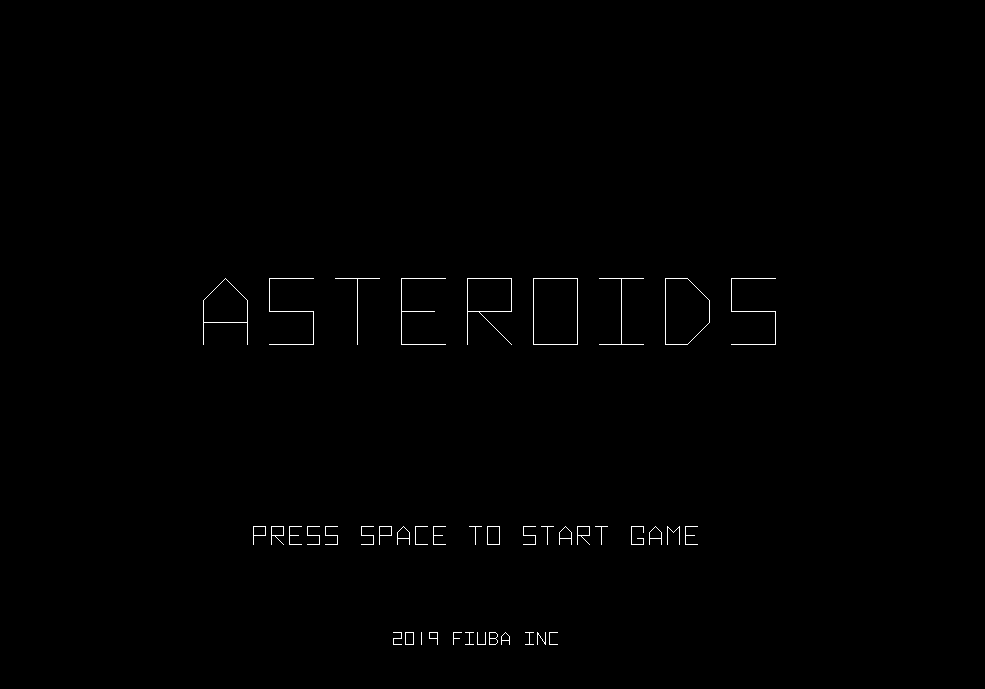
\includegraphics[width=11cm]{start_screen}
	\caption{Pantalla de inicio del juego.}
\end{figure}

Se confeccionaron dos pantallas de inicio. Una para el comienzo del juego, donde se observa el nombre del mismo, junto con las instrucciones del inicio de la primera partida jugada (Figura 1). Al iniciar, se disponen de 4 vidas, las cuales se grafican en pantalla, debajo del puntaje actual (Figura 2), para que esta
finalice, se espera a que la o el usuario pierda las vidas iniciales.
\medskip

\begin{figure}[h!]
 	\centering
	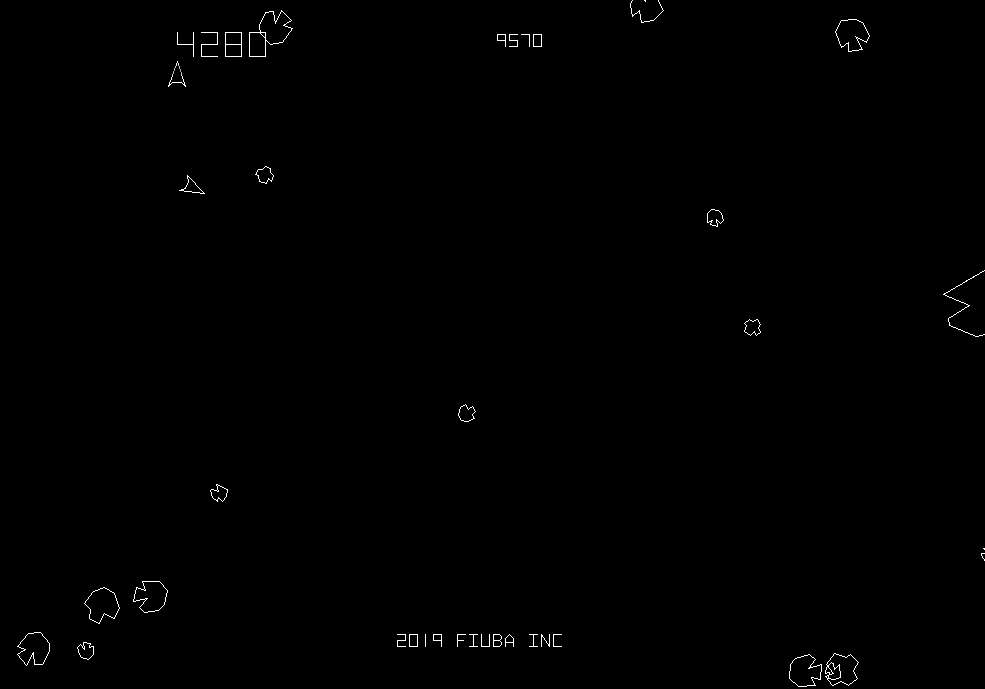
\includegraphics[width=11cm]{juego} 
	\caption{Partida en transcurso.}
\end{figure}

Una vez finalizada, se crea una pantalla de fin de partida (Figura 3), donde se proyecta el lema \textbf{GAME OVER}, junto con el puntaje recién alcanzado, y el máximo puntaje obtenido desde la ejecución del juego. Además de la condición para comenzar una nueva partida.

\begin{figure}[h!]
 	\centering
	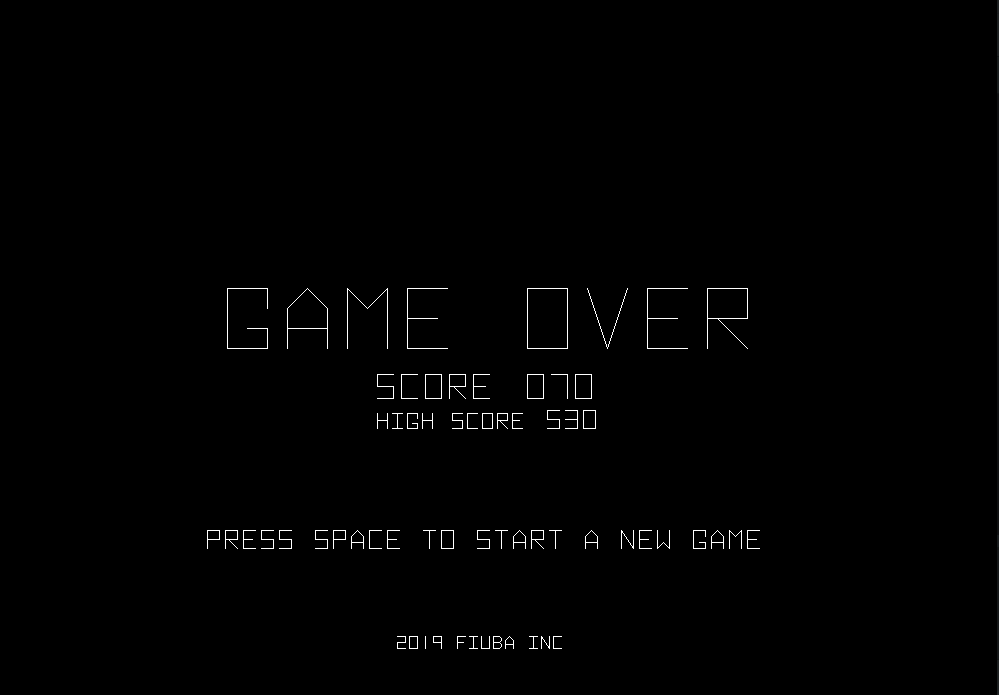
\includegraphics[width=11cm]{game_over_screen}
	\caption{Pantalla de finalización de partida.}
\end{figure} 


\section*{Dificultades}

Se han tenido diversas dificultades durante el desarrollo del juego. En un principio al implementar la función \texttt{bool graficador$\_$inicializar(const char *fn, SDL$\_$Renderer *r);}, encargada de levantar el archivo de sprites, se cometieron diversos errores respecto a su construcción. Para poder solucionarlo se necesitó de una profunda comprensión del manejo de archivos binarios. Una vez implementada, se utilizó con el fin de leer los distintos tipos de sprites contenidos dentro del archivo \texttt{sprites.bin} brindado por la cátedra, siendo posteriormente almacenados cada uno en una estructura. 

\medskip
En un principio, dentro de la función mencionada, se llamó a la función \texttt{realloc();} para tener como resultado un vector redimensionado el cual contenía las distintas estructuras de sprites, luego de evualuar 
las posibles implementaciones, optamos por adicionar los mismos a una lista local al módulo, sin la necesidad de utilizar un vector redimensionado.

\medskip
Otra de las dificultades abordadas fue cómo encarar la modularización del proyecto, por malinterpretar cuestiones
del enunciado, en un comienzo se utilizaron listas dentro de los TDAs Disparos y Asteroides, complejizando mucho más el desarrollo del código. Así que, luego de consultar las dudas, se replanteó y corrigió la estrategia de modularización.

\end{document}